%%
%% ACS project dissertation template.
%%
%% Currently designed for printing two-sided, but if you prefer to
%% print single-sided just remove ",twoside,openright" from the
%% \documentclass[] line below.
%%
%%
%%   SMH, May 2010.


\documentclass[a4paper,12pt,twoside,openright]{report}


%%
%% EDIT THE BELOW TO CUSTOMIZE
%%

\def\authorname{Tom M. Read Cutting\xspace}
\def\authorcollege{Downing College\xspace}
\def\authoremail{tr395@cam.ac.uk}
\def\dissertationtitle{Heterogeneous type checking in multi-language CPU-GPU systems}
\def\wordcount{6461}


\usepackage{array,color,epsfig,float,inconsolata,graphicx,hyperref,listings,parskip,setspace,tabularx,tabu,textcomp,xspace}
\graphicspath{ {images/} }

\newfloat{lstfloat}{htbp}{lop}
\floatname{lstfloat}{Listing}
\def\lstfloatautorefname{Listing} % needed for hyperref/auroref

\definecolor{codegreen}{rgb}{0,0.6,0}
\definecolor{codegray}{rgb}{0.5,0.5,0.5}
\definecolor{codepurple}{rgb}{0.58,0,0.82}
\definecolor{backcolour}{rgb}{0.95,0.95,0.92}
\lstdefinestyle{mystyle}{
    backgroundcolor=\color{backcolour},
    commentstyle=\color{codegreen},
    keywordstyle=\color{magenta},
    numberstyle=\tiny\color{codegray},
    stringstyle=\color{codepurple},
    basicstyle=\ttfamily\footnotesize,
    breakatwhitespace=false,
    breaklines=true,
    captionpos=b,
    keepspaces=true,
    numbers=left,
    numbersep=5pt,
    showspaces=false,
    showstringspaces=false,
    showtabs=false,
    tabsize=2
}

\lstset{style=mystyle}

%% START OF DOCUMENT
\begin{document}


%% FRONTMATTER (TITLE PAGE, DECLARATION, ABSTRACT, ETC)
\pagestyle{empty}
\singlespacing
% title page information
\begin{titlepage}

\begin{center}
\noindent
\huge
\dissertationtitle \\
\vspace*{\stretch{1}}
\end{center}

\begin{center}
\noindent
\huge
\authorname \\
\Large
\authorcollege      \\[24pt]

\includegraphics{CUni3.eps}
\end{center}

\vspace{24pt}

\begin{center}
\noindent
\large
{\it A dissertation submitted to the University of Cambridge \\
in partial fulfilment of the requirements for \\
Computer Science Tripos, Part III}
\vspace*{\stretch{1}}
\end{center}

\begin{center}
\noindent
University of Cambridge \\
Department of Computer Science and Technology \\
William Gates Building  \\
15 JJ Thomson Avenue    \\
Cambridge CB3 0FD       \\
{\sc United Kingdom}    \\
\end{center}

\begin{center}
\noindent
Email: \authoremail \\
\end{center}

\begin{center}
\noindent
\today
\end{center}

\end{titlepage}

\newpage
\vspace*{\fill}

\onehalfspacing
\newpage
{\Huge \bf Declaration}

\vspace{24pt}

I \authorname of \authorcollege, being a candidate for the M.Phil in
Advanced Computer Science, hereby declare that this report and the
work described in it are my own work, unaided except as may be
specified below, and that the report does not contain material that
has already been used to any substantial extent for a comparable
purpose.

\vspace{24pt}
Total word count: \wordcount

\vspace{60pt}
\textbf{Signed}:

\vspace{12pt}
\textbf{Date}:


\vfill

This dissertation is copyright \copyright 2018 \authorname.
\\
All trademarks used in this dissertation are hereby acknowledged.



\newpage
\vspace*{\fill}

\singlespacing
\newpage
{\Huge \bf Abstract}
\vspace{24pt}

% 1 sentence setting out the the scene, future holds promise.

% this thesis sets scene then give contributions.

% TODO: so step back and look at heterogenous computing

% TODO: because compiled in seperate languages, use better words

% 2. Paper explores cross module checking between languages.

Programming for heterogeneous architectures such as CPU-GPU systems can be
frustrating and error-prone due to the need to use incompatible programming
languages designed for different target architectures. Programmers have to
contend with manually ensuring shared data structures and types are consistent
on the boundaries between code for different architectures -- even when
targeting them with high-level and internally-sound programming languages.

There are multiple approaches that can be used to ease this burden. One
approach is to use unified languages which natively target heterogeneous
architectures. However, currently these languages are either domain-specific or
do not provide programmers the control necessary to achieve the performance
levels that traditional workflows can provide.

This paper explores and discusses the implementation of two systems for
cross-module type checking between languages. These systems each target
components of heterogeneous computing systems without sacrificing the
performance modern systems provide. Although the ideas are applicable to
general heterogeneous systems, the focus for this paper is on type checking
between languages which target GPUs and CPUs.

The first system for cross-module checking is a front-end pre-processor for the
C and GLSL programming languages to ensure the compile-time type-safety of the
data transferred between them. The second system is a pair of distinct
programming languages with compatible type systems. Both of these approaches
have their own pros and cons, with the goal of improving the user experience of
programming for heterogeneous architectures relative to the status quo, whilst
still offering the level of control that traditional workflows provide. This is
done so that runtime performance is not compromised at all.

We demonstrate how common errors that can occur when programming for GPUs using
C and GLSL are caught by the cross-module type checking systems. We then show
how these systems can be used to write many sound C and GLSL programs with
identical runtime performance to their unchecked counterparts.

\newpage
\vspace*{\fill}


\pagenumbering{roman}
\setcounter{page}{0}
\pagestyle{plain}
\tableofcontents
% \listoffigures
% \listoftables

\onehalfspacing

%% START OF MAIN TEXT

\chapter{Introduction}
\pagenumbering{arabic}
\setcounter{page}{1}

This chapter provides the motivation for the work this paper presents:
Outlining the problem, why it is important and why it has not yet been solved.
This is followed by a brief description of the two solutions presented in this
paper: a cross-module annotation checker and two languages with a unified
cross-module type checker. Finally, an overview of the entire document is
provided.

\section{Terminology}

Useful terms and domain-specific jargon are briefly explained below. Although
the concepts here are explored in depth in Chapter
\ref{chp:technical_background}, this serves as a quick reference. Finally, the
end of this section quickly clarifies common points of confusion.

\begin{itemize}

    \item \textbf{GPU:} This is a \textit{Graphical Processing Unit}, and is a
    piece of hardware that performs computations using a massively parallel
    architecture (see Section \ref{sec:gpu_hardware}. GPUs are always
    controlled by the CPU through an API, which the CPU uses to manage GPU
    resources and load code onto the GPU. The RAM a GPU directly accesses is
    called VRAM. Although computing architectures do exist where the CPU and
    GPU share access to a single pool of memory, in most architectures data
    must be explicitly transferred from the CPU's RAM to the GPU's VRAM through
    a bus.

    \item \textbf{Shader/Kernel:} A \textit{shader} is \textit{any} computer
    program written for the GPU. These are named \textit{shaders} because they
    were originally used for shading computer graphics images, but the term now
    applies to all GPU programs including those which are not related to
    graphics at all \footnote{The original specification for the first OpenGL
    shading language discusses how this decision was made \cite{GLSL_1_10}.} A
    \textit{kernel} is a name used for a computer program that runs on any
    non-CPU \textit{accelerator}, and is a term that is widely used for general
    purpose heterogeneous computing. We will use the term \textit{shader}
    within this dissertation, as both of these refer to the same concept, with
    the term differing depending on the domain.

    \item \textbf{Shading langauge:} These are programming languages that are
    used to write shaders. These are usually distinct languages from those used
    to write programs for the CPU. In the world of high performance computing
    these can also be called \textbf{kernel languages}.

    \item \textbf{Host language/code:} Programming languages and the resulting
    code which is written for and runs on the CPU. \textbf{Host} will also be
    used as a synonym for the CPU.

    \item \textbf{3D graphics library:} These are libraries for the CPU,
    commonly written in C. They provide helpful functions for graphics
    programmers and additionally provide appropriate APIs for interfacing with
    the GPU in order to render 3D graphics. This includes function and API
    calls to load and run shaders on the GPU, which are implemented by the
    drivers for GPUs.

    \item \textbf{Compute platform:} These are libraries and ecosystems similar
    to 3D graphics libraries. Although they serve the same purpose as graphics
    libraries of allowing programmers to interface with and load programs onto
    the GPU, they are designed with a focus on general purpose GPU
    computations. Additionally, some compute platforms are designed for
    hardware beyond GPUs.

    \item \textbf{OpenGL/Direct3D:} These are 3D graphics libraries. The first
    is an open standard maintained by the Khronos Group, and the
    latter is Microsoft's proprietary 3D graphics API supported by Windows
    platforms \cite{OpenGL} \cite{Direct3D}.

    \item \textbf{GLSL/HLSL:} These are \textit{shading languages}. GLSL is the
    language OpenGL uses whilst HLSL is the equivalent found in Direct3D.
    Traditionally, these languages are packaged as source-code with software
    that has been written to use them (such as a game). GPU vendors are
    responsible for writing drivers which compile source-code down to GPU
    machine-code at run-time.

    \item \textbf{OpenCL/CUDA:} These are \textit{compute platforms}. OpenCL is
    an open standard for the ``parallel programming of heterogeneous systems'',
    whilst CUDA is a similar, proprietary system that is only compatible with
    NVIDIA GPUs \cite{OpenCL} \cite{CUDA}. \textbf{OpenCL C} and \textbf{CUDA}
    are the names of the shader languages these platforms use.

    \item \textbf{Vulkan:} This is 3D graphics library \textit{and} compute
    platform that is a successor to both OpenGL and OpenCL \cite{Vulkan}. It
    differs from OpenGL and OpenCL in creating a unified approach for
    interacting with GPUs at a much lower level than those libraries. Although
    it has seen uptake in the gaming industry, it has so far had little success
    in fields where OpenCL or CUDA have traditionally been used \cite{TODO}
    \cite{TODO}. \textbf{Metal} is a similar proprietary library by Apple
    \cite{Metal}.

    \item \textbf{SPIR-V}: This is an intermediate language that is supported
    by OpenCL, OpenGL and Vulkan. The benefit of it is that graphics drivers
    only have to support interpreting this language instead of parsing a
    high-level language such as GLSL or OpenCL C. The Khronos Group hopes that
    this will spur the development of many varieties of GPU-targeted languages,
    similar to how there are many languages which compile to CPU machine-code
    \cite{SPIRV}. \textbf{OpenCL C++} is such a language that has been
    successfully developed as a result \cite{OpenCLCPPWhitePaper}.

    % \item \textbf{Framerate:} The rate at which a piece of software can render
    % a new frame in real-time. Higher is better.

    % \item \textbf{FPS:} Frames-per-second, a unit of measurement used to
    % quantify the framerate of some software. Due to the refresh-rates of most
    % consumer displays, 30FPS and 60FPS are common framerate targets.

\end{itemize}


Because heterogeneous programming is such a young field there are points of
confusion. For example, many papers creating custom interfaces or languages
claim to create ``OpenCL Code'' in their backend \cite{JITGPU} \cite{Lime2012}.
However, \textit{there is no such thing}. OpenCL is an API, and has
traditionally defined a C-like language called \textit{OpenCL C} as the
standard for writing compute kernels. Host code can then load it onto
heterogeneous devices using the OpenCL API. Many papers will output code in
this langauge for GPUs as a backend, as traditionally this has been the only
option available (aside from proprietary backends such as CUDA for NVIDIA
GPUs). In a recent development, SPIR-V can now be targeted as a back-end by
compilers instead of \textit{OpenCL C}. However, SPIR-V has yet to be targeted
by many new front-ends apart from \textit{OpenCL C++}
\cite{OpenCLCPPWhitePaper}.

\section{Motivation}

% This section introduces how a slow-down in ``Moore's Law'' has led to GPUs
% becoming increasingly relevant as more industries have turned to using them due
% to the the increased floating point computing power they provide relative to
% CPUs. However, I then explain how despite sizeable number of developers using
% GPUs, standards and standard practices are few and far between -- with a brief
% exploration of how legacy APIs, proprietary technologies have led to an
% unfortunate amount of fragmentation and steep learning curves for using GPUs.
% This is an important problem to work on due to the benefits solutions could
% provide to the wide number of developers programming for GPUs.

% NOTE: THIS SECTION HAS NOT BEEN MODIFIED (MUCH) SINCE LAST READ.

% TODO(Rewrite):

Graphical Processing Units (GPUs) can provide significant gains in
floating-point computing power relative to CPUs due to their highly parallel
nature \cite{CPUGPUOverTime}. This has lead to a growth in the use of GPUs for
general purpose computations (known as GPGPU). Whilst GPUs were originally
designed for rendering the graphics of games using a fixed-function pipeline,
changes in their design over time have made them increasingly programmable.
These design changes were driven by the desire of game developers to have
increasingly realistic, complex and diverse graphics in their games.
Furthermore, this has allowed GPUs to be used in a broadening domain of
applications, including machine learning, scientific computing, and bitcoin
mining \cite{GPUCrypto} \cite{GPUScientificComputing} \cite{GPUAI}. Section
\ref{sec:history_gpu} provides more details on this.

However despite this growth, the traditional toolchains used to program GPUs
still suffer from many of the problems they did when originally used by
graphics programmers in the early-to-mid 2000s:

\begin{itemize}

    \item Unless using C/C++ as the host langauge, the layout of data
    structures must be defined separately in both shaders and the host
    language, with erroneous behaviour if they differ.

    \item Shader functions are identified by the CPU using strings, with no
    compile-time mechanisms available to ensure that they are correct.

    % \item TODO(Content) find more errors which are not addressed by this paper
    % (such as texture mis-match).

\end{itemize}

A large root-cause of these problems is the fact that regardless of the API
used, the programs written for GPUs (known as \textit{shaders}) have to be
developed in a separate environment using high-level langauges based on C.
Therefore although data is shared between the CPU and GPU via a bus, the
programmer has to manually ensure that the data structures used to encode that
data is consistent between the programs written for the GPU and CPU.

\begin{lstfloat}
\begin{center} C$^\sharp$ \end{center}
\begin{lstlisting}[language=C]
// C# struct definition
public struct WaveParticle
{
    public Vector2 origin;
    public Vector2 velocity;
    public float amplitude;
    public float dispersionAngle;
    public int startingFrame;
}
\end{lstlisting}
\begin{center} HLSL \end{center}
\begin{lstlisting}[language=C]
//HLSL struct definition
struct WaveParticle {
    float2 origin;
    float2 velocity;
    float amplitude;
    float dispersionAngle;
    int startingFrame;
};
\end{lstlisting}
\caption{The same data structure defined separately in C$^\sharp$ and HLSL. It
is worth noting that this is much less of an issue when using C as a host
language. This is because most shading languages are based on C, so they are
able to share header files.}
\label{lst:c_sharp_hlsl_struct_comparison}
\end{lstfloat}

Listing \ref{lst:c_sharp_hlsl_struct_comparison} demonstrates a simple example
of this kind of issue, extracted from a simple GPU-accelerated water-wave
simulator \cite{WaveParticlesGPU}. In this example, units of distortion on the
surface of a liquid are represented using a data structure known as a
\textit{Wave Particle} \cite{WaveParticlesOriginalPaper}. The CPU handles
in-world physics which result in these particles being generated. However, the
GPU is used to simulate the particles themselves and additionally calculates
the shape of the resulting surface they represent before rendering the results
as shown in Figure \ref{fig:waveparticles_example}. In this case, C$^\sharp$
was the language used to write code for the CPU, and HLSL was the language used
to write shaders for the GPU. Therefore, even though both languages share the
same data structure, it has to separately be defined in both languages. If
these definitions do not agree with each other, there are no in-built
mechanisms to catch the errors this causes, at run-time or otherwise. The
outcome of such a is simply undefined runtime behaviour. Section
\ref{sec:api_challanges} fleshes out how in detail how the APIs used to write
programs for GPUs work, and demonstrates other examples of how errors such as
these can occur.


% TODO(Helpful): workout if this section is relevant.
% It is worth noting that the problems described here are further complicated by
% the fact that there are competing graphics API ``standards'', which can be
% either ``open'' or locked to a single platform \cite{OpenGL} \cite{Vulkan}
% \cite{Direct3D} \cite{Metal}. There can be different versions of the same
% standard on the same platform \cite{OpenGLHistory}. There can be different
% implementations of the same standards for different hardware on the same
% platform \cite{NVIDIADrivers} \cite{NVIDIADrivers}. There can be different
% implementations of the same standards for the \textit{same} hardware on
% different platforms \cite{OpenGLGettingStarted}. Platform and hardware
% variations can support different features and extensions, both within the
% ``open'' ecosystems \cite{VulkanExtensions} or using proprietary mechanisms
% \cite{PhysXSDK} \cite{HairworksAMD}. Furthermore, developers can be expected to
% use different toolchains depending on their use-cases
% \cite{KhronosDeveloperOverview}. Finally, GPU vendors will put game-specific
% optimisations and workarounds in their drivers so that those specific games
% will perform well on their graphics cards \cite{WhyGamesAreWorseOnLinux}.
% Therefore, games using standard APIs incorrectly, may work fine on GPUs from
% one vendor but not on GPUs from the other \cite{TODO}. Section
% \ref{sec:api_options} gives an extensive breakdown of what is summarised here.

\begin{figure}[h]
\centering
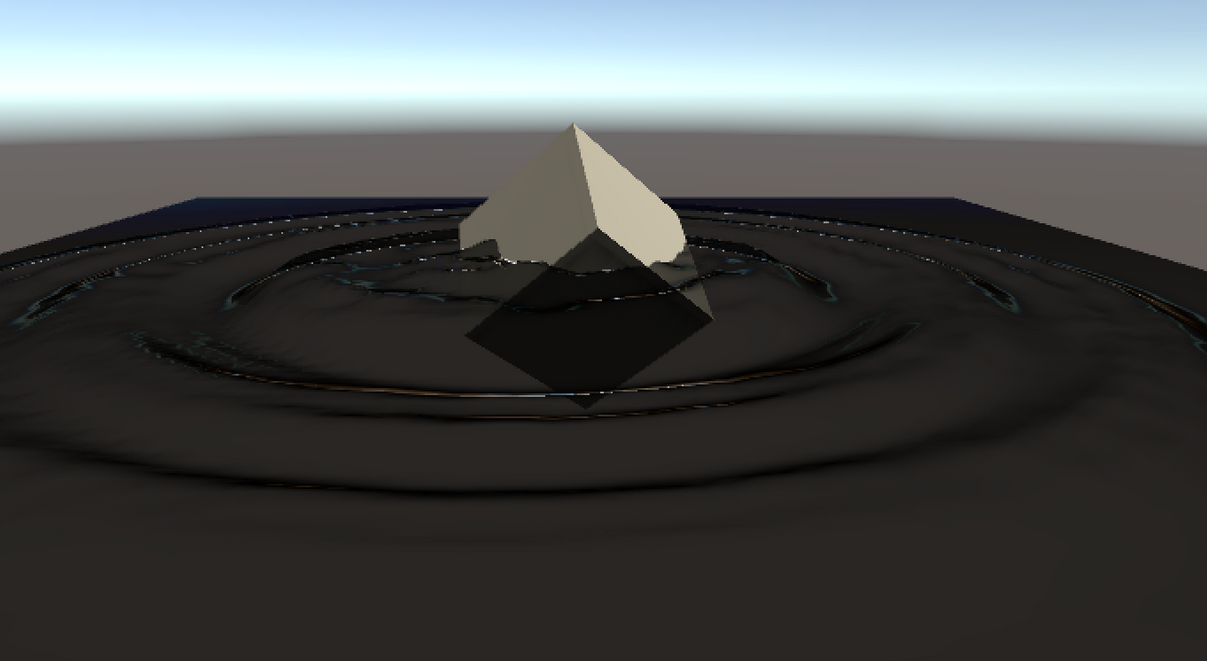
\includegraphics[width=0.8\linewidth]{waveparticles_example}
\caption{The output of wave particles system as demonstrated in the paper.}
\label{fig:waveparticles_example}
\end{figure}

There has been research into pushing forward the state-of-the-art in developing
code for heterogeneous platforms in more programmer-friendly ways. However, as
covered in Section \ref{sec:related_work}, much of the research has either been
domain-specific or provided abstractions which have an unacceptable performance
overhead for many use-cases involving GPUs. For example, a common approach is
to design a unified language which can be compiled to a run-time that supports
GPUs, as is the case with Lime \cite{Lime2010}. However, by hiding the details
of the heterogeneous backends the language targets, there is an unavoidable
run-time overhead. Working with current toolchains is an odd mix of using an
API and writing code in a GPU-specific language -- research has primarily
focused on hiding the API and simplifying GPU-specific elements by designing
unified languages abstract those details. We aim to demonstrate that
alternative approaches which improve aspects of current toolchains do exist.

We have provided the motivation for the solutions described in this paper,
first by demonstrating the prevalence of GPUs and how important improvements to
toolchains which target them could be. Secondly, we have demonstrated the
problems current toolchains face with a brief example showing how data
structures must be defined separately in programming languages for the GPU and
the CPU. Finally, we provided a brief explanation of why research has yet to
tackle these problems.

\section{The Solutions}

\label{sec:solutions_introduction}

This section introduces the two systems this paper presents as solutions to the
problems described above. First by describing what the desired outcomes of
those solutions should be and then how they should improve over the status quo.
This is followed by the solutions themselves; first describing the annotation
processor and then the pair of languages with a unified type system. The pros
and cons of each are then discussed to round off the section.

\subsection{Desired Outcome}

As described in Section \ref{sec:related_work}, systems which aim to improve
over current toolchains often the sacrifice the control that traditional
workflows provide in order to improve the user-experience that programmers
have. The issue with this approach is the fact that performance is still
important in many domains where GPUs are used -- to the point where programmers
still choose to make the trade-off of working directly with APIs like OpenGL or
Vulkan instead of choosing the usability that abstractions could otherwise
provide \cite{TODO}. Therefore, solutions which aim to build and improve upon
the status quo should provide all the options that traditional toolchains do,
including exposing any underlying graphics or compute APIs.

Although this means these solutions are limited in the abstractions that they
can provide, there are some ``easy wins'' to be made. This is demonstrated by
the example problem shown in Listing \ref{lst:c_sharp_hlsl_struct_comparison}
and elaborated on in Section \ref{sec:api_challanges}. Bugs may easily be
introduced to due errors in using the API; these can prevented by compile-time
checks. That is, instead of trying to unify code that is written for the CPU
and GPU under a single language or system which is designed to abstract-away
API calls (thereby reducing the possibility of introducing errors as the
compiler generates API calls for the programmer), we can acknowledge that these
targets are different enough to justify writing host code and shaders in
different programming languages. However, we can use compile-time type checking
\textit{between} these languages and compile-time checks on the API calls
\textit{themselves} in order to have the compiler catch errors which would
otherwise be left undetected.

In conclusion, any solution that aims to improve upon current programming
models should deliver the benefits described above without sacrificing anything
current toolchains provide. This can be done by targetting specific classes of
errors as described in Section \ref{sec:api_challanges}. We can do this with
two techniques: compile-time cross-language checks and the processing of
annotations to check the validity of raw API calls.

\subsection{What was done}

We created two systems for checking programs across language boundaries in
CPU-GPU systems. Each one of these systems is focused on demonstrating a
different approach to implementing compile-time cross-language checks and
checking the validity of raw API calls for graphics programming. We chose to
target the Vulkan API to demonstrate that these ideas can work at the lowest
low-level. However, the ideas are also applicable to other APIs such as OpenGL,
OpenCL or Direct3D.

The first system is a pre-processor for C and GLSL that operates on annotated
sections of code. The goal here was to demonstrate how an existing pair of
languages with similar type systems could be extended in order to have
error-checking on raw API calls. Furthermore, as C and GLSL are one of the most
language-pairings for graphics programming, this was done to show how a lot of
existing code could stand to benefit from these techniques.

The second system is a proof-of-concept pair of languages with the features
provided by the pre-processing system baked-into the type system at the
language level. We had two goals with this. The first was to demonstrate that
such a system could work. The second was to show how existing high-level
languages could be extended with a shader-language. This would be suitable for
a language such as C$^\sharp$, which has a strong type system, but is
compromised and arguably \textit{less safe} than C when using shaders. This is
because C and GLSL can share code as they have similar syntax. $C^\sharp$ and
GLSL do not have similar syntax, meaning that the problem shown in Listing
\ref{lst:c_sharp_hlsl_struct_comparison} becomes a problem. Due to resource
limitations, we designed a pair of languages from scratch with the minimum
subset of features required in order to demonstrate that this is possible,
instead of extending an existing full-features language such as $C^\sharp$.

One thing to note is that our goal was not to write a comprehensive set of
tools which could be used to catch all errors of this nature at compile-time.
We instead hope to demonstrate some ideas which could be used to catch
many-kinds of errors, by demonstrating implementations of two systems which
have been designed to capture a small subset of them.

\subsubsection{Annotation System}

The annotation system is a command line program that takes annotated code
written in C and annotated code written in GLSL as input. An example annotation
and the code that is generated is shown in Listings
\ref{lst:annotation_example_input} and \ref{lst:annotation_example_output}.

\begin{lstfloat}
\begin{center} Annotated C \end{center}
\begin{lstlisting}[language=C]
VkComputePipelineCreateInfo compute_pipeline_create_info = {
    .sType = VK_STRUCTURE_TYPE_COMPUTE_PIPELINE_CREATE_INFO,
    .pNext = 0,
    .flags = 0,
    .stage = @create_verification(
        struct: VkComputePipelineCreateInfo,
        name: "test_shader",
        data: {
            .stage = VK_SHADER_STAGE_COMPUTE_BIT,
            .module = shader_module,
            .pName = "main"
        }
    ),
    .layout = pipeline_layout,
    .basePipelineHandle = 0,
    .basePipelineIndex = 0
};
VkPipeline pipeline;
vkCreateComputePipelines(
    vulkan_device, 0, 1, &compute_pipeline_create_info,
    0, &pipeline
);
\end{lstlisting}
\begin{center} Annotated GLSL \end{center}
\begin{lstlisting}[language=C]
@verify(from: "test_shader", function:
void main() {
    output_buffer.values[gl_GlobalInvocationID.x] = input_buffer.values[gl_GlobalInvocationID.x];
})
\end{lstlisting}
\caption{Annotated C and GLSL, the output for these snippets (without
annotations) is shown in Listing \ref{lst:annotation_example_output}. The full
example can be found on the project GitHub repository \cite{ProjectSource}.}
\label{lst:annotation_example_input}
\end{lstfloat}

Listing \ref{lst:annotation_example_input} shows an example of an API call that
can result in an error that could be checked-for at compile-time. In this case
the running of a shader named \texttt{main}. Here, the host code makes the
\texttt{vkCreateComputePipelines} API call in order to create a compute
pipeline\footnote{This is just an API call that needs to be made in order to
run a computer shader on the GPU \cite{TODO}} \cite{vkCreateComputePipelines}.
An instance of the \texttt{VkComputePipelineCreateInfo} struct containing a
\texttt{VkPipelineShaderStageCreateInfo} struct is passed to that API call,
which ultimately specifies which function in the shader to use within the
compute pipeline \cite{VkComputePipelineCreateInfo}
\cite{VkPipelineShaderStageCreateInfo}. Annotations are used to label the
creation of the \texttt{VkPipelineShaderStageCreateInfo} structure on the host
and the \texttt{main} function within the shader using the
\texttt{@create\_verification} and \texttt{@verify} commands respectively. The
annotation itself is given a name, \texttt{"test\_shader"} which both the host
code and shader reference. The annotation processor takes annotated code as
input, and produces output similar to Listing
\ref{lst:annotation_example_output}.

\begin{lstfloat}
\begin{center} Output C \end{center}
\begin{lstlisting}[language=C]
VkComputePipelineCreateInfo compute_pipeline_create_info = {
    .sType = VK_STRUCTURE_TYPE_COMPUTE_PIPELINE_CREATE_INFO,
    .pNext = 0,
    .flags = 0,
    .stage = {
        .sType = VK_STRUCTURE_TYPE_PIPELINE_SHADER_STAGE_CREATE_INFO,
        .pNext = 0,
        .flags = 0,
        .stage = VK_SHADER_STAGE_COMPUTE_BIT,
        .module = shader_module,
        .pName = "main",
        .pSpecializationInfo = 0
    },
    .layout = pipeline_layout,
    .basePipelineHandle = 0,
    .basePipelineIndex = 0
};
VkPipeline pipeline;
vkCreateComputePipelines(
    vulkan_device, 0, 1, &compute_pipeline_create_info,
    0, &pipeline
);
\end{lstlisting}
\begin{center} Output GLSL \end{center}
\begin{lstlisting}[language=C]
void main()
{
    output_buffer.values[gl_GlobalInvocationID.x] = input_buffer.values[gl_GlobalInvocationID.x];
}
\end{lstlisting}
\caption{The output generated by Listing \ref{lst:annotation_example_input}. The full
example can be found on the project GitHub repository \cite{ProjectSource}.}
\label{lst:annotation_example_output}
\end{lstfloat}

The annotation provides two key features in this particular example. The first
is the generation of boiler-plate for the creation of the
\texttt{VkPipelineShaderStageCreateInfo} struct. This was done to investigate
boiler-plate generation features a pre-processor could provide. The second and
most important key feature is the compile-time checking of the function name --
ensuring that \texttt{main} cannot be renamed in the host or shader without
being consistently renamed in the other. If we were to ensure such an error was
introduced in raw C and GLSL, the resulting behaviour would be a runtime error.
However, not all inconsistencies which can be checked like this result in
runtime errors, others can simply result in incorrect or undefined runtime
results, so these ideas could be even more helpful when expanded to these
problems.

This example demonstrates how potential runtime errors or incorrect runtime
behaviour can be detected through the usage of annotations which are checked at
compile-time using a pre-processor. The flexibility of this system is that the
programmer can remove the annotations if they desire, especially if they are
using complex runtime features. However, this system can still be used to help
ensure that an initial implementation is correct. Furthermore, Section
\ref{sec:design_annotation_processor} covers design decisions that were made
with typical shader workflows in mind such that annotations can be kept for
most use-cases.

\subsubsection{New Set of Languages}

The new set of languages takes the form of a compiler that can compile code
written in two related langauges which are each designed to target different
architectures. The first language, called \textit{the host langauge}, is a
language that is designed to be compiled for the CPU. The second language,
called the \textit{the shader langauge} is similarly designed to target GPUs.

% TODO(Content!): Massively expand!

The goal here was to leverage the opportunities intermediate shader languages
present. Section TODO(Content) explains how historically compiling custom
langauges to shaders has been a difficult endeavour, due to a plethora of
inconsistencies between the implementation of shader languages by different GPU
vendors. Intermediate shader langauges help solve this problem.

% TODO(Task): Read https://www.khronos.org/registry/spir-v/specs/1.0/SPIRV.pdf

Listing \ref{lst:language_example} shows the same snippet of code as the
annotation example shown in Listing \ref{lst:annotation_example_input}.

\begin{lstfloat}
\begin{center} Host Language \end{center}
\begin{lstlisting}[language=C]
let shader_interface :Shader_Interface = @define_shader_interface(name="main");
let compute_pipeline_create_info: [] C::VkComputePipelineCreateInfo = [{
    sType = VK_STRUCTURE_TYPE_COMPUTE_PIPELINE_CREATE_INFO,
    pNext = 0,
    flags = 0,
    stage = get_VkPipelineShaderStageCreateInfo(
        shader_interface=shader_interface
    ),
    layout = pipeline_layout,
    basePipelineHandle = 0,
    basePipelineIndex = 0
}];
var pipeline : C::VkPipeline;
C::vkCreateComputePipelines(
    device=vulkan_device,
    pipelineCache=0, createInfoCount=length(compute_pipeline_create_info),
    pCreateInfos=get_c_ptr_from_array(compute_pipeline_create_info),
    pAllocator=null,
    pPipelines=&pipeline
);
\end{lstlisting}
\begin{center}
Shader Language
\end{center}
\begin{lstlisting}[language=C]
let main() {
    output_buffer.values[gl_GlobalInvocationID.x] =
        input_buffer.values[gl_GlobalInvocationID.x];
}
\end{lstlisting}
\caption{The output generated by Listing \ref{lst:annotation_example_input}. The full
example can be found on the project GitHub repository \cite{ProjectSource}.}
\label{lst:language_example}
\end{lstfloat}


\subsection{Pros and Cons}

These approaches naturally have their own pros and cons relative to each other
and relative to other related work in the field (Section
\ref{sec:related_work}).

Compared with using raw graphics APIs, these techniques present an obvious
benefit: they reduce the likelyhood of certain classes of errors from being
made. However, they do potentially cost of friction.

\begin{itemize}

    \item PROS:

        \item Reduce friction

        \item Help Me s

\end{itemize}

\section{Overview}

% This is the introduction where you should introduce your work.  In
% general the thing to aim for here is to describe a little bit of the
% context for your work -- why did you do it (motivation), what was the
% hoped-for outcome (aims) -- as well as trying to give a brief
% overview of what you actually did.

% It's often useful to bring forward some ``highlights'' into
% this chapter (e.g.\ some particularly compelling results, or
% a particularly interesting finding).

% It's also traditional to give an outline of the rest of the
% document, although without care this can appear formulaic
% and tedious. Your call.

TODO(Content!): Give overview of paper.

\section{Summary}

TODO(Content!): summarise introduction.

\chapter{Technical Background}

\label{chp:technical_background}

% A more extensive coverage of what's required to understand your
% work. In general you should assume the reader has a good undergraduate
% degree in computer science, but is not necessarily an expert in
% the particular area you've been working on. Hence this chapter
% may need to summarize some ``text book'' material.

% This is not something you'd normally require in an academic paper,
% and it may not be appropriate for your particular circumstances.
% Indeed, in some cases it's possible to cover all of the ``background''
% material either in the introduction or at appropriate places in
% the rest of the dissertation.

% This chapter covers relevant (and typically, recent) research
% which you build upon (or improve upon). There are two complementary
% goals for this chapter:
% \begin{enumerate}
%   \item to show that you know and understand the state of the art; and
%   \item to put your work in context
% \end{enumerate}

% Ideally you can tackle both together by providing a critique of
% related work, and describing what is insufficient (and how you do
% better!)

% The related work chapter should usually come either near the front or
% near the back of the dissertation. The advantage of the former is that
% you get to build the argument for why your work is important before
% presenting your solution(s) in later chapters; the advantage of the
% latter is that don't have to forward reference to your solution too
% much. The correct choice will depend on what you're writing up, and
% your own personal preference.

We introduce what a GPU is and how it is a good benchark for heterogeneous
hardware in general. We then provide extensive coverage of the relevant history
of graphics hardware and how it developed over time to become useful in many
fields beyond real-time rendering in video games. Following that, a breakdown
of graphics APIs is provided, to give both the context for the problem this
paper aims to tackle and the underlying technology the solutions depend upon.
Then, the difficulties and issues with programming for GPUs is summarised from
the contents of this chapter with a brief explanation of which ones the
solutions presented in this paper aim to tackle and which ones they do not. The
chapter finishes of with an overview of related research in this area,
demonstrating both were they succeed and how they fail to tackle the specific
problems that are solved here.

% TODO(Citation): Why low level details are important (eg unified memory versus seperate
% memory)
% https://www.slideshare.net/zlatan4177/gpgpu-algorithms-in-games
% https://en.wikipedia.org/wiki/Heterogeneous_System_Architecture

\section{The GPU}

\label{sec:gpu_hardware}

TODO(Content!):

\begin{center}
\begin{tabular}{||c||c|c|c||}
\hline
        & Number of Cores  & FLOPS                                         & Type of parallelism \\
\hline
\hline
CPU     & 1 - O(10)        & Up to 1 Teraflop \cite{IntelTeraFlop}         & TODO                \\
\hline
GPU     & O(10) - O(10000) & Up to 100 Teraflops \cite{NVIDIA100TeraFlops} & TODO                \\
\hline
\end{tabular}
\end{center}

% Can be worth being wary of GPU vs CPU performance based on performance alone.
% http://people.eecs.berkeley.edu/~sangjin/2013/02/12/CPU-GPU-comparison.html


\section{A (brief) History of GPU computing}

\label{sec:history_gpu}

Graphics Processing Units (GPUs) were originally fixed-function hardware
accelerators for 3D rendering aimed at hobbyist gamers who desired hardware to
play games with the most complex graphics possible. They really took off after
GLQuake demonstrated the improvements dedicated 3D graphics hardware could
achieve relative to CPUs \cite{GLQuake}. Since then, due to rapid developments
and competition, the scope and capabilities of graphics cards has expanded such
that they are the highly-parallel general computation machines we find them to
be today. However, the developments GPUs experienced weren't pre-planned, and
despite their current general-purpose nature, the terminology surrounding
graphics cards has its foundation in graphics. Furthermore, as the industry has
been so volatile, standards around using GPUs and heterogeneous hardware are
still solidifying, with many fragmented communities and confusion around the
future roadmap of both graphics and compute APIs.

This section summarises relevant milestones related to the history of
heterogeneous computing in order to help the reader understand why the field is
in its present state. However, it is not comprehensive and excludes many
details.

% \caption{
% Tabulated history of graphics APIs and graphics card development. Naturally
% this tabled misses many details, especially related to the earlier years when
% there were many hardware vendors, the graphics market was volatile, and there
% were many, many competing graphics APIs each with their own extensions and
% features. Futhermore, the introduction of certain features are really hard to
% pin-down. For example, there is no set-date where GPUs went from being
% fixed-function hardware to becoming programmable hardware. Changes such as
% these happened gradually, with extra configurability being slowly introduced to
% graphics hardware with extensions and additional API calls until shading
% languages needed to be defined in order to program these configurations more
% systematically. However, even these languages were limited in their
% capabilities and support for advanced features like loops and flow-control took
% time to be introduced into hardware.
% }
% \end{table}

\begin{itemize}

    \item 1992 \textbf{OpenGL 1.0} released by Silicon Graphics (SGI) as an API
    for interacting with graphics hardware on 3D graphics workstations. OpenGL
    was created from their proprietary ``IrisGL'' API in order to prevent
    competitors from creating their own proprietary graphics APIs and
    fragmenting the market. The API allowed users to issue basic commands in
    order to set-up 3D scenes, apply basic fixed-function lighting, and then
    render the scenes \cite{OpenGL_1_0}. Control of the OpenGL specification
    eventually transfers from SGI to various owners before landing in the hands
    of the \textbf{Khronos Group} \cite{OpenGL}.

    \item 1996 \textbf{Direct3D 2.0} release by Microsoft, so named, because it
    was the \textit{first} version of Direct3D. Although at this point API was
    designed as an abstraction for a software renderer
    \cite{JohnCarmackPlanDirect3DvsOpenGl}, it eventually developed into an API
    for interfacing with graphics cards.

    \item 1996 \textbf{3Dfx Voodoo1} graphics card released. Although not the
    first graphics card, it dominated the consumer market and brought 3D
    graphics rendering to the mainstream \cite{Voodoo1}.

    \item 1999 \textbf{NVIDIA GeForce 256} released; the first video card to be
    called a \textbf{GPU}. It was the first consumer-PC graphics hardware to
    accelerate ``transform and lighting'' operations, allowing them to
    offloaded form the CPU. The ``transform and lighting'' component of GPUs
    prefigured what would eventually run shaders \cite{GeForce256}.

    \item 2000 \textbf{The Khronos Group} founded to provide structure for open
    standards in 3D graphics. Reflecting the increasing flexibility of graphics
    cards over time, they now also provide standards virtual and augmented
    reality, heterogeneous computing, computer vision, parallel computing and
    neural networks \cite{KhronosGroupAbout}. In 2006 control of OpenGL was
    transferred to the Khronos Group \cite{OpenGLToKhronos}.

    \item 2001 \textbf{GPGPU}, \textit{general purpose computations on GPUs},
    are demonstrated by Larson and McAllister. They perform fast matrix
    multiplications by encoding the matrices as the inputs and outputs of the
    graphics pipeline such that the graphics pipeline can then be configured to
    perform the desired calculations \cite{MatrixGPU}. Subsequent papers then
    show how GPUs can outperform CPUs for many operations that are desirable in
    scientific computing \cite{CUDAtoOpenCL} \cite{Kruger03linearalgebra}
    \cite{LUGPU} \cite{SparsematrixGPU}.

    \item 2003 \textbf{OpenGL ES}, \textit{OpenGL for embedded systems},
    released by the Khronos Group \cite{OpenGLESRelease}. It is currently the
    most widely deployed 3D graphics API in history, being popular on mobile
    platforms such as Google's Android operating system \cite{OpenGLES}.

    \item 2004 \textbf{GLSL} (also known as OpenGL Shading Language or glslang)
    introduced into the \textbf{OpenGL 2.0} specification. It was created to
    tame the complexity and proliferation of custom OpenGL extensions with
    assembly languages that customised parts of the fixed-function pipeline.
    This formally replaced parts of the graphics pipeline with
    user-programmable stages which were defined using a hardware-independent
    high-level language (replacing proprietary assembler languages that
    individual GPU manufacturers were introducing). GLSL at this point was
    defined as \textit{two} closely-related shading languages for different
    parts of the pipeline: the vertex processor (for modifying vertices) and
    the fragment processor (for modifying the final image). Finally, the
    language was forward-looking in supporting many features that hardware at
    the time did not \cite{GLSL_1_10}.

    \item 2005 \textbf{Unified Shader Architecture} introduced in ATI's
    \textbf{Xenos GPU}, released as part of the Xbox 360. The ``vertex'' and
    ``pixel'' segments of the GPU pipeline are unified into a single component
    that can run either. This brought GPUs closer to being highly-parallel
    general computation machines and away from being direct fixed-function
    hardware implementations of the graphics pipeline represented by APIs such
    as OpenGL \cite{XenosDemystified}. All GPUs would soon adopt this
    architecture \cite{HistoryOfTheGPU}.

    \item 2006 \textbf{CUDA} (Compute Unified Device Architecture) introduced
    by NVIDIA as a parallel computation platform and API. This allowed
    programmers to exploit the \textbf{GPGPU} capabilities of graphics hardware
    directly, without having to encode data as the input and output of the
    OpenGL pipeline. This made GPU computing more efficient and accessible
    \cite{AboutCUDA}.

    \item 2008 \textbf{Open CL} platform developed and announced by Apple as a
    potential open standard for GPGPU computing. Existing as a distinct entity
    from OpenGL, it has its own shader language called \textbf{OpenCL C}. Apple
    handed control of the OpenCL specification to the Khronos Group, with the
    first implementation of the standard releasing alongside the Snow Leopard
    OS X update in 2009 \cite{OpenCL}. OpenCL also added support other
    heterogeneous architectures such as DSPs and FPGAs.

    \item 2015 \textbf{SPIR-V} shading language released alongside
    \textbf{OpenCL 2.1} \cite{SPIRVLaunch}. Unlike the high-level
    \textit{OpenCL C} and \textit{GLSL} shading languages which drivers need to
    compile themselves, this is an intermediate language based on \textit{LLVM
    IR} which compilers for any language can target. \cite{LLVMIR}
    \cite{SPIRV}. SPIR-V support was then added to \textbf{OpenGL 4.6} and
    supported by Vulkan at launch, unifying the shading langauges of Khronos'
    APIs \cite{SPIRVOpenGL}.

    \item 2016 \textbf{Vulkan} released by the Khronos Group. A low level
    graphics and compute API for graphics cards that aims to better represent
    how modern graphics cards are designed, this differs from OpenGL, whose
    abstraction of a traditional graphics pipeline no longer represents the
    unified nature of GPUs \cite{VulkanAnnouncement}. Unlike OpenGL and OpenGL
    ES, Vulkan is the same on both desktop, mobile and embedded systems
    \cite{Vulkan}.

\end{itemize}


The capabilities of GPUs and their related APIs have massively expanded since
they were both introduced. This has allowed GPUs to be used in increasingly
general domains, including scientific computing, crypto-currency mining,
high-frequency trading, and artificial intelligence \cite{GPUCrypto}
\cite{GPUScientificComputing} \cite{GPUTrading} \cite{GPUAI}. Some hobbyists
for home the cards were originally designed are even being priced out of the
market \cite{GPUCrypto} \cite{BitcoinRuiningPricing}. However, there are many
different standards and APIs for different use-cases of the same hardware as a
result of a complex history. Furthermore, many of these use-cases have
widely-used proprietary alternatives such as CUDA, DirectX, Metal and even
proprietary game console APIs \cite{CUDA} \cite{Metal} \cite{Direct3D}
\cite{PS4PortCrew}. However, with the release of SPIR-V, aspects of the various
Khronos Standards are converging. Additionally, despite a foundation in
graphics, the compute capabilities of Vulkan are expanding such that OpenCL
could eventually be merged into the API \cite{VulkanOpenCLMerge}. Furthermore,
the low-level nature of new graphics and compute APIs such a Vulkan, Metal and
DirectX 12 have allowed portability initiatives to bring implementations of
those APIs as light shims above the others \cite{VulkanPortabilityInitiative}
\cite{VulkanPortabilityInitiativeAnnouncement}.

\section{The Challenges with the APIs}

\label{sec:api_challanges}

% TODO(Content) mention how Vulkan is merging the OpenGL, OpenCL and OpenGL ES.

% TODO(Helpful): Good comparison of mess vs potential future (Unity Pipeline).
% http://www.g-truc.net/doc/2015%20-%20EuroLLVM%20-%20SPIR-V.pdf
% can also be shown in conclusion.

Due to the complex history of GPUs and their APIs as described in Section
\ref{sec:history_gpu}, the APIs used to interact with GPUs naturally have many
issues as many of them have evolved over the course of many years. However,
this situation has recently improved with the creation of the Vulkan graphics
and compute API. This is a very low-level API that has been designed from the
ground-up to reflect the way modern GPUs \textit{actually} operate
\cite{Vulkan}. This contrasts with graphics APIs like OpenGL, which reflect how
GPUs \textit{historically} operated \cite{TODO}. Therefore, this section is not
going to enumerate all of the issues graphics APIs have, but instead will
briefly describe the workflow and toolchains of using a graphics or compute
API, and then enumerate the challenges our systems aim to ease.

A comprehensive overview of the challenges graphics and compute API present is
given in Appendix \ref{app:other_API_issues}.

\subsection{An overview of a typical graphics or compute API}

% A graphics API is what programmers use in order to make a GPU render the
% graphics they desire, usually outputting the results to a display. Popular
% graphics APIs include OpenGL, OpenGL ES and DirectX. Due to how the nature of
% the hardware that makes GPUs suitable for rendering operations, they are also
% incredibly adept at performing certain kinds of general purpose computations.
% Using GPUs for these kind of computations is called GPGPU computing. Graphics
% APIs now expose some of these compute capabilities, as they can be useful for
% rendering and even performing other operations (such as physics, or procedural
% generation \cite{TODO}) as a part of the rendering pipeline. However, as the
% traditional graphics pipeline is quite heavyweight, alternative APIs for
% interacting with GPUs have been developed which are targeted towards
% programmers who only which to perform GPGPU computations. These are called
% compute APIs. Popular compute APIs include OpenCL and CUDA. All of these APIs
% are normally implemented at the driver-level of graphics hardware.

% Naturally, having two distinct sets of APIs for interacting with the same
% hardware is not ideal. As it would be akin to having to use two different ISAs
% depending on the domain a particular applications was being designed for.
% Therefore there has been movement towards developing low-level APIs which will
% eventually be capable of filling both roles. Vulkan is one such API.

A compute or graphics API typically consists of two components: the API itself
and a ``shader''/``kernel'' language that is used to write programs that run on
the GPU itself. The API will typically come in the form of a C library, with
functions that the user can call in order to direct an abstracted model of the
GPU to perform specific operations. Some of those API calls enable the user to
load their shaders onto the GPU, transfer data to the GPU, and then execute the
shaders on that data. Historically, most, if not all, shaders and kernel
language have been heavily based on the C-programming langauge. This has had a
few benefits and drawbacks:

Benefits include:

\begin{itemize}

    \item Writing shaders is relatively straightforward if you are familiar with
    a C-like language.

    \item If C/C++ is the host language, data structures can be shared by
    including the same header file in shaders and host code.

    \item Having a standardised high-level language helps ensure that the same
    shaders will run on hardware from a variety of different vendors.

    \item Since all of the languages are based on C, porting code from one
    shader language to another can even be done by simply performing ``find and
    replace'' operations \cite{PS4PortCrew}.

\end{itemize}

Drawbacks include:

\begin{itemize}

    \item High-level language specifications can be ambiguous, which means
    drivers can implement the same standard in incompatible ways \cite{TODO}.

    \item Unlike popular CPU compilers such as clang and gcc, the compilers
    that drivers use are not-only proprietary but developed by much smaller
    teams. This can lead to bugs where even fuzzing programs with changes which
    should result in identical outcomes results in breaking the output
    \cite{GLFuzz}. %TODO(Helpful): maybe include an image of this

    \item Applications must be distributed with the high-level source-code to
    these shaders, meaning the shaders themselves must be tokenised, parsed,
    type-checked, compiled and optimised at run-time \cite{TODO}.

    \item If the host-language is in a language with enough syntactic
    differences from the shader languages, data-structures must be defined in
    both languages (Listing \ref{lst:c_sharp_hlsl_struct_comparison}).
    Furthermore, there are no built-in mechanisms to ensure these definitions
    are consistent - even at run-time.

    \item The C type system is limited compared with more modern programming
    languages. So even when using C and a C-based shader language, many things
    remain unchecked (Section \ref{sec:issues_summary}.

    \item As the drivers have their own optimisation systems, code does need to
    be tuned for specific hardware if you want to maximise performance
    \cite{TODO}.

    \item Cross-compiling is difficult, as optimisation can depend on specific
    tweaks and implementations of the same shading language can be
    incompatible. This has resulted in the same shading C-based shading
    langauges being used, even when host-code is written in something
    completely different \cite{TODO}.

\end{itemize}

These problems still exist, however, the keys to potentially solving many of
them are appearing. The first step towards this is the creation of the SPIR-V
intermediate language \cite{SPIRV}. This is a language that has been designed
to better represent the low-level instructions GPUs actually use. Therefore,
drivers need to simply translate these instructions, as opposed to compiling a
high-level language. The goal here is to reduce the number of implementation
bugs that have previously occurred \cite{TODO}. Additionally, reference
language \textit{specifications} can be replaced by a reference language
\textit{compiler}, which can be open-source and therefore receive input from
many more individuals. Additionally, the same front-end is now used regardless
of which hardware code will eventually be compiled for, resulting in much more
consistent behaviour. As the behaviour of the intermediate language itself is
more consistent on different platforms configurations, it can be targetted by
different languages with more stability. An optimiser of the intermediate
langauge itself can also be shared. The reference compiler has also enabled the
creation of more-complex shading languages, such as the creation of
\textit{OpenCL C++}, which would have been much harder to create if each
hardware vendor had to write their own compilers for this language within their
drivers. This is a shader language based on C++ that allows programmers to use
many of C++'s features. Therefore more code can be shared between the host and
shader, in addition to the advanced type checking features C++ provides over C.
Finally, the same compiler can be shared by the \textit{shader language},
OpenCL C++, and the ``single-source'' heterogeneous computing system known as
SYCL. SYCL is a way of writing code for heterogeneous hardware within C++, such
that the compiler then automatically generates the necessary API calls to run
that code on heterogeneous hardware. This abstracts many aspects of
heterogeneous computing in order to make programming for GPUs easier, however
programmers do sacrifice the control they would otherwise have if they wanted
to achieve optimal performance. However, by having SYCL and OpenCL C++ share
the same compiler, the SYCL and OpenCL communities can much more easily share
code, and migrating between these systems is now possible without having to
re-write all of the code that has been written for heterogeneous hardware.

Furthermore, this intermediate language is used by OpenGL, OpenCL and Vulkan,
meaning new shader/kernel languages can target a single back-end in order to
target many APIs. Furthermore, the Vulkan portability initiative allows
developers to run Vulkan on-top-of different APIs on platforms which may not
natively support Vulkan itself \cite{TODO}. This will hopefully result in an
ecosystem which much more closely resembles the ``hourglass model'' that CPUs
enjoy today. %TODO(Helpful) cite unity presentation slide.

Cross-compiling between different intermediate languages for different APIs is
easier than doing the same for high-level languages \cite{TODO}.

Part of this project aims to capitalise on this recent development in GPU
computing, with the demonstration of a custom language for the CPU which has a
shader-language counterpart. This demonstration is with multiple goals in mind:

\begin{itemize}

    \item To demonstrate the possibilities that SPIR-V presents in allowing any
    high-level language to have its own shading language. This means that the
    issue demonstrated in Listing \ref{lst:c_sharp_hlsl_struct_comparison}
    need no-longer exist.

    \item To demonstrate how a language which is designed with GPUs as a
    first-class citizens can have a type-system which results in less
    error-prone programming for the GPU. However, unlike many other
    such-languages, explicit API calls can still be made, ensuring programmers
    still have they control they need in order to optimise code how they would
    like.

\end{itemize}

Although \textit{OpenCL C++} has demonstrated some of this, it does have a few
limitations. The first is that fact that it is only compatible with OpenCL.
Although the SPIR-V backend is shared by OpenGL, OpenCL and Vulkan, OpenCL is
the only API which has enjoyed the creation of a high level shader language
such as OpenCL C++. OpenGL and Vulkan still use GLSL, which is a C-like
language with the limitations that incurs. This project aims to demonstrate how
such a language can target graphics APIs as well. C++ does not treat GPUs as
first-class citizens, therefore OpenCL C++ has to be designed with the existing
capabilities of C++ in-mind. This project aims to demonstrate features that a
language could provide if it is aware of the interactions between shader and
host languages.

\subsection{Issues Summary}

\label{sec:issues_summary}

This section enumerates the specific issues the project aims to solve. This
project consists of two systems, an annotation system for C and GLSL and a
custom pair of programming langauges. Although there is overlap in which
problems they aim to solve, they differ in their approaches. The approaches
they each take will be briefly described. Furthermore, some of the issues are
only tackled by one of the systems, in this case that will be mentioned.

The examples listed here are taken from various sources. Due to the limited
space available, only the relevant fragments of these sources are displayed.
TODO(Content): List those sources, and provide a reference to a complete summary of
them (maybe put into appendix).

\subsubsection{Issue 1: Redefining Datastructures}

This issue is demonstrated in Listing \ref{lst:c_sharp_hlsl_struct_comparison}
and is extremely common when writing host code in a language that differs
significantly from C.

A common example is wanting to run a shader which takes a buffer of structs as
input or output. When using C/C++ as the host language, you do not really have
any problems, because most common shader langauges are based on C. Therefore,
you can define a struct in a \texttt{.h} header file and include it in both
your shader and host code.

An issue arises when host code is written in another language that is distinct
from C. In this case, when using shaders, you have to define the datastructure
in both the host and the shader langauge separately. This is what Listing
\ref{lst:c_sharp_hlsl_struct_comparison} demonstrates.

Errors can easily occur when these representations of the same datastructure
differ. For example, given different definitions, if the CPU fills a buffer
with a given datastructure and then transfers it to the GPU for it to operate
on, the resulting behaviour will simply be incorrect. Debugging these kind of
errors is hard, as there are no runtime or compile time checks, so a programmer
has to locate it by manual inspection.

Futhermore, this is not a niche error. For example, the Unity game engine uses
C$^\sharp$ as a scripting language, whilst using HLSL for shaders \cite{TODO}.
Between April and July 2015, Unity applications from over 170,000 developers
were installed on mobile hardware alone \cite{UnityByTheNumbers}.

We hope to demonstrate how this issue could be tackled through the development
of a pair of custom languages. We aim to demonstrate how a language that differs
from C can have a shader language derived from it, so that these errors can
be avoided. For example, going forward, it could be possible to write shaders
in Unity using a shader language based on C$^\sharp$ instead of one based on C.

The reason this has not been previously possible, is because of TODO(Content): find
other sections explaining why and reference them.

\subsubsection{Issue 2: Refering to kernel/shader names using strings}

This issue is demonstrated in Listing \ref{lst:annotation_example_output}.

Running a shader consists of multiple steps, the following are important and
relevant to this problem. Firstly, a shader needs to be written and saved in a
file. Then, depending on the API, the shader may need to be compiled into an
intermediary format in order to run on the GPU. Then, when the application is
running, it performs three important steps. First, it passes a pointer to the
the shader data to the API, so that it can handle loading the code onto the
GPU. Second, it identifies which kernel (essentially a function) within that
code should be run. Third, it then makes an API call to run that kernel.

However, this has an issue, and that is that the kernel is identified by a
string, as shown in Listing \ref{lst:annotation_example_output}, and there are
no compile-time checks between the shader and the host code in order to make
sure that the host code identifies a kernel that actually exists. As there is
no direct link between the string that the host code uses to identify the
kernel and the name of the kernel itself, refactoring and renaming kernels can
be tricky.

For example, misnaming the kernel in Vulkan, causes a
\texttt{VK\_ERROR\_INVALID\_SHADER\_NV} error at runtime.

% https://www.khronos.org/registry/vulkan/specs/1.1-extensions/man/html/vkCreateComputePipelines.html

% https://www.khronos.org/registry/vulkan/specs/1.1-extensions/man/html/VkResult.html

The annotation system and the new langauges both aim to catch these errors at
compile-time using different mechanisms.

% \subsubsection{Issue 3: Texture Business}

% Another issue is that of

% \begin{figure}[h]
% \centering
% 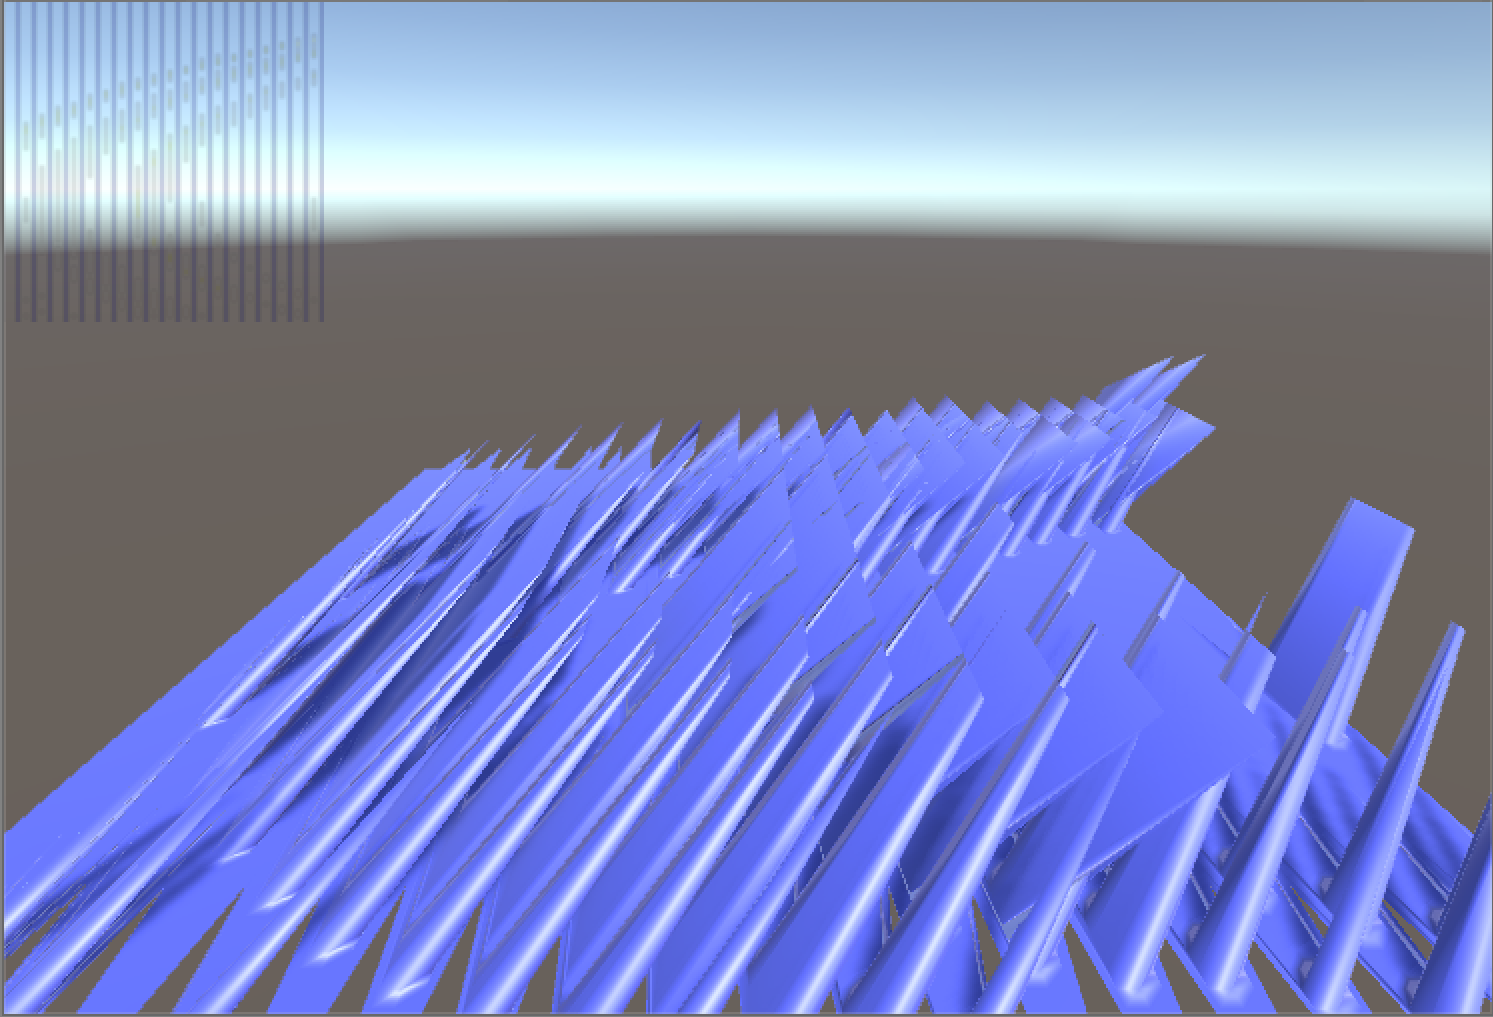
\includegraphics[width=0.8\linewidth]{texture_copy_issues}
% \caption{An error caused by incompatible texture definitions.}
% \label{fig:texture_copy_issues}
% \end{figure}

% Figure \ref{fig:texture_copy_issues} demonstrates the issue.


% \subsubsection{Issue 4: Uninitialised Data}

% TODO(Helpful): write it out

% \begin{lstfloat}
% \begin{lstlisting}[language=C]
% const float fixedDeltaTime;
% const int currentFrame;
% const float particleSpeed;
% float2 getPosition(int startingFrame, float2 velocity, float2 origin) {
%     float t = (fixedDeltaTime * (float)(currentFrame - startingFrame));
%     return origin + (t * particleSpeed * velocity);
% }

% const int horiRes;
% const int vertRes;
% const float planeWidth;
% const float planeHeight;
% StructuredBuffer<WaveParticle> waveParticleBuffer;
% RWTexture2D<float4> amplitudeTexture;

% ///
% /// Splat the wave particles to the splatTexture
% ///
% #pragma kernel SplatParticles
% [numthreads(THREAD_GROUPS_X, 1, 1)]
% void DrawParticles(uint3 id : SV_DispatchThreadID)
% {
%     WaveParticle particle = waveParticleBuffer[id.x];
%     float2 waveParticlePosition = getPosition(
%         particle.startingFrame, particle.velocity, particle.origin
%     );
%     int xPos = (int)round((waveParticlePosition.x / planeWidth) * horiRes);
%     int yPos = (int)round((waveParticlePosition.y / planeHeight) * vertRes);
%     amplitudeTexture[int2(xPos, yPos)] +=
%         float4(0.0, particle.amplitude, 0.0, 0.0);
% }
% \end{lstlisting}
% \label{lst:draw_particles}
% \caption{An example of an HLSL computer shader that takes a particle stored in
% in a buffer and copies its amplitude to a specific location on a texture.}
% \end{lstfloat}

\section{Related Work}

\label{sec:related_work}

This section describes related work in the field of modifying or improving GPU
toolchains beyond traditional low-level libraries. It aims to show the diverse
set of approaches that have been taken to doing this and the progress that has
been made, in addition to demonstrating that the specific problems targeted by
this paper have yet to be addressed.

Since the creation of the SPIR-V intermediate language for heterogeneous
programming (as discussed in Chapter \ref{chp:technical_background}), some
progress has been made in simplifying and unifying how GPUs are interacted with
for compute purposes. For example the Khronos Group have recently standardised
a modified version of C++, \textit{OpenCL C++} for developing compute kernels
\cite{OpenCL22Release} \cite{OpenCLCPPWhitePaper} \cite{OpenCL}. This has only
been possible because it can be compiled to SPIR-V, whereas previously graphics
drivers had to implement OpenCL C directly, limiting how complex OpenCL's
shader language could become. However, despite unifying some aspects of host
and accelerator languages, this uses the traditional workflow of programming
compute kernels and host code separately, with no cross-module checking at the
API boundaries \cite{OpenCL22Release}.

SYCL is a framework by the Khronos Group built on top of OpenCL that abstracts
away the API calls to enable ``single-source'' C++ development which
automatically generates host and kernel code from a single C++ source file
\cite{OpenCL22Release} \cite{SYCL}. SYCL has seen uptake in terms of multiple
implementations \cite{ComputeCPP} \cite{triSYCL}, and has been adopted as a
backend for various machine learning frameworks such as TensorFlow and Eigen
\cite{SYCLTensorFlow} \cite{SYCLEigen}. However, this approach does have its
limitations in removing the ability for developers to control how those API
calls are made. Both OpenCL and SYCL are also limited in only being suitable
for \textit{compute} applications, and do not allow for the graphics operations
that GPUs are capable of. However, Vulkan and OpenCL could merge in the future,
which may open the door to this happening \cite{VulkanOpenCLMerge}.

Research has been done to make GPU and heterogeneous computing available in
high-level dynamic languages. Theano and TensorFlow do this by abstracting a
compute platform such as OpenCL or CUDA using a framework or library
\cite{Theano2016} \cite{TensorFlowWhitePaper}. This technique has primarily
seen success in scientific computing and machine learning. Others have created
custom high-level languages which target GPUs directly. Harlan, developed by
Holk et al., is a domain-specific langauge (DSL) based on Scheme for GPUS, with
support for higher order programming with Scheme-influenced syntax and
semantics \cite{Harlan} \cite{HarlanAnnouncement}. GPipe extends the functional
language Haskell such that shaders can be written functionally and OpenGL calls
can be made in type-safe ways, however, the garbage-collected nature of Haskell
makes it unsuitable for many of the domains GPUs are used in such as games
\cite{HaskellState} \cite{GPipe}. Halide is a DSL for image processing and
computational photography \cite{Halide}. Fumero et al. have developed
techniques to automatically offload computation from high-level interpreted
dynamic languages using just-in-time compilation to achieving speedups by
compiling R to an OpenCL C backend \cite{JITGPU}. Futhark is an attempt to
design a functional data-parallel array language from the ground-up that can
target GPUs, targeting an OpenCL backend \cite{Futhark}.

Existing langauges have also been extended with the functionality to compile
parts of their programs to heterogeneous architectures. Lime and JCUDA take the
approach of compiling Java or Java-like code in such a manner \cite{Lime2010}
\cite{Lime2012} \cite{JCUDA2009}. However, they differ in their approaches.
Lime aims to abstract low-level details of heterogeneous computing such that
arbitrary backends can be targeted, including GPUs (using OpenCL as a back-end)
and FPGA synthesisation. JCUDA targets CUDA, allowing CUDA programs to be
created using Java, with an interface that aims to closely match CUDA's native
C API. OpenACC is a system specifically targeted at scientists that lets
programmers mark appropriate sections of normal C++, C or Fortran code as
possible candidates for accelerated parallel computation \cite{OpenACC}. The
goal is specifically to allow users to write code as they normally would for
the CPU, and then add directives to code fragments as hints to the compiler
that those fragments could perform optimally if run on a GPU.

Another approach has that has been taken is to abstract away underlying APIs
such as CUDA and OpenCL with platforms that can target both as backends. HIP is
a project that does this by allowing CUDA code to be compiled to C++ that uses
an abstracted API so that developers can convert their CUDA projects to
something that can target arbitrary backends \cite{HIP}.

In addition to SYCL and OpenCL C++, there have been other attempts at bringing
heterogeneous programming models natively to C++ through parallel programming
standards. C++ AMP is a C++ library, programming model, and compiler developed
by Microsoft that targets DirectX 11 \cite{CAMP}. However, it seems to have
died \cite{CAMPFail1} \cite{CAMPFail2}. \textit{C++ extensions for parallelism}
has brought such standards to the C++ standard template library
\cite{CPPParallelism}. Finally, OpenMP is an API standard dedicated to
shared-memory multiprocessing \cite{OpenMP}. HCC is a project aims to take C++
code that conforms to any of these standards and compile it to AMD's GCN
instruction set \cite{HCC}.

As can be seen, there has been progress in making programming for heterogeneous
architectures easier. However, the focus has been primarily on GPGPU computing.
Futhermore, although the creation of SPIR-V and Vulkan are slowly changing
this, all of these systems have had to target fairly-high level backend APIs
such as OpenCL or CUDA, in addition to languages interpreted by device drivers
such as \textit{OpenCL C} or \textit{CUDA C/C++}, which has limited the
performance and stability of the higher-level systems \cite{GLFuzz}.
Additionally, apart from \textit{Open CL C++}, these all either present
alternate high-level interfaces or abstract them away in order to ensure
simplified and less error-prone programs. This differs from the approach taken
here, which is to mark-up low-level API calls directly, so that they are
checked at compile-time for consistency without sacrificing the control that
would otherwise be lost by abstractions. Furthermore, we targeted both
\textit{compute} and \textit{graphics} back-ends, as opposed to focusing only
on compute.

% TODO(Helpful): Future roadmap confusion

% TODO(Helpful): Vulkan Validation Layers

\chapter{Design}

The project is composed of two systems. The first is a pre-processing system for
C and GLSL that ensures the enforcement of interfaces between the two
languages. The second is a set of two novel toy languages which natively
support such enforcement. How these are used is described in Section
\ref{sec:solutions_introduction}

\section{Design Goals}

The ultimate design goal of the cross-module type checking systems is to make
programming for GPUs less frustrating and error prone by catching errors which
can commonly occur. However, unlike other systems which do this, we cannot have
\textit{any} compromises to runtime performance relative to existing industry
standards such as GLSL and OpenGL. This includes not limiting the possible
programs programmers can make. Naturally there pros and cons to this approach.

There are other concerns beyond performance that need to be taken into account
which inform the design the system. For example, a commonly used feature is too
\textit{swap} shaders with identical interfaces in-and-out at runtime.
Therefore this needs to be supported by the system as well.

\begin{itemize}

    \item Having a non-intrusive system

    \item supporting simple workflows, but without sacrificing control

    \item Allow different shaders to be type-checked at compile-time but
    swapped in-and-out at run-time.

    \item Allow custom wrappers to exist.

    \item Generalise to different APIs.

\end{itemize}

\section{Workflow}

One of the important parts of the system is the implementation of the workflow.

\subsection{Targeting Vulkan}

We decided to target the Vulkan graphics and compute API in the implementation
of our systems \cite{Vulkan}. Done for the following reasons:

\begin{itemize}

    \item Vulkan is a modern graphics API with runtime safety-features (such as
    validation layers) that other APIs such as OpenGL lack \cite{TODO}. Our
    goal was to demonstrate how even a modern graphics API could suffer from
    the issues described in Section \ref{sec:api_challanges}, and how our
    systems could introduce compile-time checks for these errors.

    \item Vulkan is already being widely used in the gaming industry, so the
    use cases described here are applicable to a wide audience.
    %TODO(Helpful) : phrase better).

    \item Vulkan is a low-level API. One of the goals of our systems was to
    demonstrate how they have no runtime overhead, this is done by allowing
    users to make Vulkan API-calls directly.

\end{itemize}

\subsubsection{Build Strategy}

Due to the fact that they aim to solve similar problems, both the annotation
processor and compiler have a similar build strategy in order to ensure that
they work with typical shader workflows and toolchains.

One of the reasons it is hard to check the consistency between shaders and host
code is the fact that shaders are loaded onto the GPU by the CPU at run-time
using API calls. Systems such as SYCL circumvent this problem by using
``single-source'' programming models - users write their shaders and host-code
in a single file, and the appropriate API calls are generated by the compiler
\cite{TODO}. As the compiler is in control of which code does get loaded-in at
run-time, it can ensure that cross-language interactions are consistent.
However, in addition to preventing optimisations that could be made to the API
calls, this system does have a few other limitations: one of them being able to
swap and load shaders at run-time based on arbitrary logic.

Being able to do this is important for two reasons: the first is for allowing
users to easily change which shaders render their applications. For example, a
game could have a high-quality shader that implements a realistic lighting
model for rendering, and a low-quality shader that is less realistic, but can
run on weaker hardware. Being able to change these is important for users who
wish to compare the differences. The second reason arbitrary runtime shader
loading is important, is in allowing artists to quickly iterate shaders
themselves. When designing shaders, being able to ``hot-load'' shaders is very
important. If a project needed to be re-compiled every time a shader was
modified, that would massively impede productivity.

Therefore we take a novel approach in type checking between CPU and GPU code.
Firstly, shaders and host code are written in different files, using different
langauges in the traditional manner. However, the host code is analysed using a
program which generates metadata at the compile-time of the host code. This
approach does have limitations: it relies on the programmer to correctly
mark-up their CPU code so that the errors can be checked-for. However, the
benefit of this is that raw-and-unchecked API calls always exists as an option.
This system does not impose any limitations on existing workflows.

This metadata can then be fed as input when the GPU code is compiled. Which can
be at some arbitrary point after the CPU code is compiled, or even when the
application itself is running. This metadata can be used to ensure that the
shaders which are being written, are consistent with what the CPU expects when
making API calls to load it into the GPU.

\section{Annotation System}

\label{sec:design_annotation_processor}

The annotation system is designed to demonstrate how existing graphics
workflows using C and a C-like shader can be improved in order to be less
error-prone, without compromising on the control they provide. Furthermore, the
lessons learned from designing and implementing it influenced the design of the
pair of languages which provide these benefits natively as described in Section
\ref{sec:design_langauges}. The annotation system is specifically designed to
make the errors described in Section \ref{sec:api_challanges} as hard as
possible. Although Vulkan uses SPIR-V as an intermediate shader langauge, most
programmers use the open-source GLSL-to-SPIR-V compiler to write high-level
shaders \cite{TODO}. Additionally, the Vulkan API is defined in C. For these
reasons, the decision was made to target C and GLSL using the annotation
system.

\subsection{Referring to function names using strings}

\section{Languages}

\label{sec:design_langauges}

The language is meant to demonstrate how a higher-level language than C
\textit{could} have an be designed with GPUs in mind such that a shader
language derived from it can make use of modern language features in addition
to features specifically designed to ensure programming for the GPU is less
error-prone. However, this differs from many other custom langauges which have
aimed to do this, as we are not abstracting-away any API calls. Therefore the
features these languages provide are the same as those from the annotation
system, but with them baked-in to the type-system of these languages.

Due to resource constraints, these languages do not aim to replicate
\textit{all} of the features that one would expect from an industrial language
such a Java, C, C++, C$^\sharp$, Swift, Rust, etc. They merely aim to provide
the bare-minimum feature-set needed in order to demonstrate the ideas of this
paper. They are very much toy languages.

\subsection{C-interoperability}

In order to provide zero-overhead API calls, the host-language must be able to
call directly into C. This also has an additional benefit, in that C libraries
can be leveraged in order to make up for deficiencies in the language itself.

Multiple design decisions were made in order to achieve this as easily as
possible. It is worth noting that a more robust implementation of these
languages would go about things differently. We mention if this is the case.

The first design decision that was made was to target C as the backend for the
host language. Although an intermediate language such as LLVM-IR would be the
optimal choice for a more-developed language \cite{TODO}, C was chosen as it
was easier to do in the time available. Furthermore, the output of the compiler
can in-turn be included by C-programs. This was a feature that was taken
advantage of in order to easily implement automated tests of langauge features,
by having C++ call-into code generated by the compiler \cite{AutomatedTestCode}
\cite{AutomatedTestOutput}.

The second decision was to provide a keyword for the inlining of C code in the
language. This was simplified by the fact that C was the target back-end of the
language. The reason for this was two-fold, the first being in allowing
programmers to include libraries within their code, and the second being in
providing the ability to write programs using C. This helps alleviate the fact
the host language is a limited toy language.

The third decision that was made was the creation of a special namespace for C
functions which can be called by the language. For example, if someone wishes
to call \texttt{printf}, they simply need to prepend it with \texttt{C::}, such
that they write \texttt{C::printf}. This was done so that it is clear for the
programmer when they are calling out to C, and to make it easier for the
compiler to know which names need to be mangled when compiling code.

The final decision that was made was the creation of an \texttt{@extern}
keyword which can be used to declare the existence of C-functions and structs
within included C code. This relies on the programmer to get the correct type
definitions. This was done to avoid the need to parse C in order to extract
these definitions, which would be the ideal solution. However, it does mean
that C functions can be type-checked within the language.


\begin{lstfloat}
\begin{lstlisting}[language=C]
#c_environment {
    #include<stdio.h>
}

@extern let printf(format : * const u8)

let print_fish() {
    // Note: c_str is a `magic` function that converts
    // in-langauge strings to c-strings. A mature
    // implementation would have a standard library that
    // provided this feature.
    C::printf(format = c_str(
        str = "fish"
    ));
    return;
}
\end{lstlisting}
\label{lst:lang_c_interop}

\caption{Example of C-interactions. The \texttt{\#c\_environment} keyword is
used to include the \texttt{stdio.h} header. The \texttt{@extern} is used to
mark the existence of the \texttt{printf} function and define its type. As the
language does not support variadic arguments, the full interface cannot be
represented within the language.}

\end{lstfloat}

Listing \ref{lst:lst:lang_c_interop} demonstrates an example of the features
used to interact with C.

\subsection{Shader Language}

The shader language is based on the host langauge, but differs with both
restrictions and enhancements, reflecting the capabilities of GPUs.

The biggest restriction is the lack of a \texttt{\#c\_environment} command
which can be used to embed C in the host langauge. Additionally, this means
that there is no \texttt{C} namespace which can be used to access C functions.
Futher restrictions include the inability to use certain datatypes such as
pointers and strings.

However, the shader languages has the addition of a
\texttt{\#glsl\_environment} command, which can be used to embed GLSL within
the langauge, statements which are accessed using the \texttt{GLSL} namespace.
Furthermore, the shader langauge is supplemented by the addition of basic
vector datatypes.


% TODO(Content): Add more detail once shader langauge is well defined

\subsection{Cross-Language type system}

A big benefit of these pair of languages is that they have a cross-language
type-system. This different significantly from many GPU programming models,
where the host language and the shader language differ significantly. Although
when using C or C++, existing shader languages are syntactically similar enough
to them for some code such as data structures to be shared. However, even
sharing code like this is limited, as C has a fairly limited type system.
Furthermore, there are no mechanisms for expressing within files that they are
intended to be used for both shader and host code.

We there improve over the status quo in one significant way, by allowing files
to be explicitly marked as a shared module for both our host and shader
languages. Therefore, the compiler can compile files marked in this way whilst
being aware of this fact, meaning that when shared modules are included by any
code, the compiler can emit errors if those modules do not conform to the
restricted subset of features which are available in both the host and shader
langauges.

%TODO(Content): Add more details and examples once these mechanisms are well defined.

\subsection{Other Features}

Although not directly-relevant to the problem at-hand, the language has the
following features which distinguish it from C:

\begin{itemize}

    \item Instead of declaring variables by writing \texttt{type\_name
    variable\_name = expression}, the user writes \texttt{var variable\_name :
    type\_name = expression}.

    \item Type inference is supported with the syntax \texttt{var variable\_name
    := expression}.

    \item Immutable values can be declared with \texttt{let value\_name :
    type\_name = expression}.

    \item Strings and arrays both explicitly store there own length values.

    \item Forward declarations are not needed, the compiler can lookahead for
    function and structure definitions. Futhermore, it can detect if there are
    cycles within structs automatically.

    \item Pointers in the host language can be nullable or non-nullable.
    Assigning \texttt{null} explicitly to non-nullable pointers is illegal, and
    assigning from nullable to non-nullable pointers must either be guarded or
    use an explicit cast.

\end{itemize}

\chapter{Implementation}

% This chapter may be called something else\ldots but in general
% the idea is that you have one (or a few) ``meat'' chapters which
% describe the work you did in technical detail.

The source code for the project is publicly available and open-source
\cite{ProjectSource}. The implementation is formed of two distinct components,
the C-annotation pre-processor and the custom-languages compiler. Although both
are written in C++, Python is also used as a build-system to enable simple
cross-platform builds. The project was developed and tested on both Ubuntu
16.04 and Windows 10 operating systems.

\section{Pre-processor}

The pre-processor takes the form of a commandline program, that can operate
in two modes:

\begin{itemize}

    \item \textbf{Host Mode}: indicated by the \texttt{-h} flag, allows the
    user to provide an annotated C file as input, with two outputs being given.
    The first output is indicated by the \texttt{--out-c} flag, which tells the
    annnotation processor where to output the processed C file. The second
    output is indicated by the \texttt{--out-metadata} flag, which tells the
    annotation processor where to output metadata associated with the
    annotations. This metadata is used to check GLSL files. An example command
    line instruction would be: \texttt{./annotation\_processor -h input.c
    --out-c output.c --out-metadata check.metadata}.

    \item \textbf{Shader Mode}: indicated by the \texttt{-s} flag, allows the
    user to provide annotated GLSL and metadata file as input, with GLSL being
    provided as the output, or an error, if the GLSL and the metadata are
    inconsistent. An example command line instruction would be:
    \texttt{./annotation\_processor -s input.glsl check.metadata --out-glsl
    output.glsl}.

\end{itemize}

Although the pre-processor seems simple, the intention is for it to be used as
a command-line program that can be used by more comprehensive build systems.

The annotation processor works by looking for ``\texttt{@}'' directives within
C or GLSL code. When such a directive is found, it tokenises and parses the
relevant sections of the provided input using a recursive descent parser,
creating an abstract syntax tree.

For annotated C code, the AST is semantically analysed, with a special
dataformat to store metadata which can be used to ensure that GLSL annotations
which are checked later are consistent with the annotated C.

The annotated GLSL code is checked using a similar strategy.

% TODO(Content): flesh this out more

\section{Compiler}

The compiler is a much more complex endeavor than the annotation processor, and
consists of a single program which is able to compile code written in three
languages: the host language, the shader language, and the subset of the two.
Input for the compiler is achieved in a similar manner to the input into the
annotation processor.

\subsection{Parsing multiple langauges}

The reason the different langauges share the same compiler program is to allow
for the easy sharing of code and to ensure consistency between the two.
However, by sharing the same compiler, can needs to be taken to ensure that the
compiler handles code intended for a particular backend in the desired manner.

This is achieved through the use of an internal state machine within the
recursive descent parser , where during parsing of a given input, the compiler
can be in three possible states for parsing:

\begin{itemize}

    \item \textbf{\texttt{HOST}:} When in the \texttt{HOST} state, the compiler
    ensures that it only compiles code that conforms to the host language. It
    fails, with a compilation error, if code does not conform.

    \item \textbf{\texttt{SHADER}:} When in the \texttt{SHADER} state,
    similarly, only shader language conforming code is parsed.

    \item \textbf{\texttt{SHARED}:} When in the \texttt{SHARED} state, only
    code which is of the valid subset of the host and shader langauges is
    parsed. Source files indicate themselves as shared through an
    \texttt{@shared} directive as the first token of the source file.

\end{itemize}

\subsection{Semantic Analysis}

Semantic analysis is fairly straightforward. It's done by recursing on the AST,
and regardless of the language being compiled, the same semantic analysis
algorithm is performed. However, in order to handle different types which may
be available in the different langauges, the symbol tables have different types
inserted into them when initialised. Additionally, externally declared types,
constants and functions are added to the \texttt{C} namespace for host code and
to the \texttt{GLSL} namespace for shader code.

\subsection{Intermediate Representation}

After parsing, an intermediate representation (IR) is generated from the AST.
This IR takes the form of a three-address code, stored in a quadruple format.
Both backends share the same IR, however, some opcodes are only permissable for
certain target backends. Examples of this include the \texttt{MALLOC\_OP}
instruction, which is only present for the CPU backend. Name mangling is
performed at this stage of the compilation, however, uses of functions and
types in the reserved C and GLSL namespaces for host and shader code
respectively are left untouched.

\subsection{Backends}

There are two different backends, a C backend when compiling the host langauge
and a GLSL backend when compiling the shader langauge. These are handled by
directly translating given quadruples to source code for the target langauges.
The reason for targetting these as backends is given in Section TODO(Helpful).

% \subsection{Interfacing with existing langauges}

% TODO(Helpful): reference usage of FNV hash for symbol table. \cite{FNVHash}.


\chapter{Evaluation}

% For any practical projects, you should almost certainly have
% some kind of evaluation, and it's often useful to separate
% this out into its own chapter.

In this chapter, we analyse how the two systems help prevent errors of the kind
described, which will be shown through different code snippets. Due to the
complexity of using graphics APIs, these snippets are incomplete. For example,
the host code which makes the appropriate API calls to run a simple compute
shader that copies items from one file to another is over 750 lines long
\cite{TODO}. The source for all of these examples will be referenced.


% \section{Performance}

% Ideally, there shouldn't be any performance overhead in either of the
% solutions. For the annotation processor, that's fairly straight-forward to
% establish, as it is essentially syntactic sugar that sits on-top-of C and GLSL.

% However, although the custom language has semantics very similar to C and GLSL,
% and in theory identical programs in both environments should be \textit{just
% as} performant as C - the compiler may not optimise as well as it should.

% TODO(Content!):

\section{Error-Prevention}

In this section we analyse each of the errors shown in Section
\ref{sec:sec:issues_summary}, demonstrating how both the annotation system and
custom heterogeneous languages prevent the programmer from making them.

\subsection{The Errors}

\subsubsection{Issue 1: Redefining Datastructures}

This is an issue solved by the new set of custom langauges.

TODO(Content!):

\subsubsection{Issue 2: Referring to function names using strings}

This is an issue solved by both the annotation system and the new set of custom
langauges.

TODO(Content!):

% \subsubsection{Issue 3: Texture Business}

% TODO(Helpful):

% \subsubsection{Issue 4: Uninitialised Data}

% TODO(Helpful):

\chapter{Conclusion, Further Work and the Future of Heterogeneous Programming}

% As you might imagine: summarizes the dissertation, and draws
% any conclusions. Depending on the length of your work, and
% how well you write, you may not need a summary here.

% You will generally want to draw some conclusions, and point
% to potential future work. \cite{DirectXWorkings}

We have shown two novel systems which can make programming for GPUs using
conventional low-level APIs less error-prone. The first, an annotation
processor for C and GLSL, aims to demonstrate how existing workflows which use
these langauges can be improved in this way, without sacrificing performance.
We also demonstrate a novel pair of langauges, demonstrating how modern type
systems can bring these kind of checks to GPU programming, whilst still
allowing programmers to use the low-level C APIs and writing their shaders
explicitly.

Although these techniques do work for some simple cases, there is still much
more work that could be done and places where they could be taken. Furthermore,
as covered in Section \ref{sec:api_challanges}, there are still many difficult
problems with using graphics APIs. Although these techniques only solved a
subset of them, this model could hopefully be expanded to more.

TODO(Content):

% NOTE: CURRENTLY ONLY CONTAINS SPECULATION ON THE FUTURE OF HETEROGENEOUS
% PROGRAMMING. IT IS CURRENTLY SLIGHTLY UNSTRUCTURED BUT PRESENTS THE IDEAS
% I THINK THE FINAL CONCLUSION WILL.

Something which the creation of SPIR-V enables, and that this paper
demonstrates is possible, is the ability to \textit{extend} langauges with
custom shading langauges whilst still preserving existing API interfaces. This
is different from that currently done both in industry and reasearch. For
example, whilst programs for the Unity game engine are written in C$^\sharp$,
shaders for it have to be written in HLSL \cite{TODO}. Projects such as SYCL
and LIME did extend C++ and Java respectively to allow shaders to be programmed
in their host languages, however they used optimising compilers with the goal
of abstracting away the underlying OpenCL API and outputting OpenCL C code for
shaders. However, OpenCL C++ has demonstrated that API interfaces can be
preserved whilst shaders are written in the host language
\cite{OpenCLCPPWhitePaper}. This also means that SYCL can use this compiler in
its backend \cite{TODO}.

This leads into the approach I expect other high-level languages to take in the
future as, briefly summarised below:

\begin{itemize}

    \item Port desired graphics and compute APIs such as OpenGL, OpenCL and
    Vulkan to your language so that they can be called directly from it.

    \item Create a modified extension of your language that can be used to
    program shaders, the compiler for this extension can target SPIR-V.

    \item Use any features your language may have to increase the safety of
    specific API calls using techniques similar to what has been demonstrated
    in this paper. Alternatively custom annotations may be used to strengthen
    this system.

    \item Create ``single source'' abstractions which an optimising compiler
    can use to generate appropriate API calls for your computations, taking
    advantage of your shader compiler. The relationship here can be similar to
    the one between SYCL and OpenCL C++.

\end{itemize}

The benefits of this approach is that the GPU ecosystem will more closely
resemble the ``hourglass model'' that CPUs enjoy today, instead of the separate
fragmented ecosystems it currently suffers. Eventually, the higher-level OpenCL
and OpenGL could be APIs which are implemented in terms of the lower-level
Vulkan, bringing this ``dream'' another step closer to reality
\cite{OpenGLonVulkan} \cite{VulkanOpenCLMerge} \cite{OpenGLOverload}.

% TODO(Helpful): Software renderer + Vulkan CPU for CPU side debugging


\bibliographystyle{unsrt}
\bibliography{references}

\appendix
\singlespacing

\chapter{A comprehensive overview of GPU API issues}

\label{app:other_API_issues}

Writing about some of the issues here.

This section gives an overview of the general challenges programmers face when
using graphics APIs. Firstly, the context and history of graphics APIs are
described, with a focus on OpenGL and Vulkan. Subsequently, the general
workflow of writing programs for GPUs is described, before finally the
individual problems that type heterogeneous type safety seeks to address are
identified.

Programmers interact with GPUs using APIs, however, as the development of and
growth of GPUs in computing has been relatively organic and ad-hoc, these APIs
themselves have many legacy components and can be difficult to work with
\cite{NVIDIAInternshipLessons}.

% TODO(Citation): can reference this blog:
% http://aras-p.info/blog/2015/03/13/thoughts-on-explicit-graphics-apis/
% http://aras-p.info/blog/2014/05/31/rant-about-rants-about-opengl/

To understand the challenges of working GPUs, one must first both understand
the current workflow of GPUs and how that workflow has developed over time.

The best point of comparison is the CPU, and programming for the CPU. When
programming for the CPU, programmers often have access to a plethora of
programming languages which are suited to different needs and are capable of
targeting a wide range of backends. Furthermore, the instruction sets of CPUs
are published and well-documented, allowing programmers to write applications
for them directly -- even allowing them to write their own compiler for them
if they so desire. Finally, in the world of desktop computing, x86 is the
de-facto standard architecture, massively increasing the portability of
programs which target desktop PCs without the need for hardware abstractions
which could come with performance penalties.

The workflow of the GPU is very different.

\subsection{OpenGL}

Although GPUs do not have a standard ISA, open standards for GPU computing have
been developed and maintained by the Khronos Group \cite{TODO}, which was
founded in 2000 by a group of companies for this purpose. OpenGL is the most
widely used standard graphics API that they maintain, however, the API has a
history dating back to the early 1990's \cite{TODO}, with control of the
standard being passed from Silicon Graphics in 2006 \cite{TODO}. For a long
time the OpenGL family of graphics APIs were the only cross-platform family of
graphics APIs, with OpenGL ES, a related API, being used for mobile and
embedded systems \cite{TODO}.

Despite OpenGL being an open standard with a differently-flavoured API for
non-desktop systems, portability and development using the API is difficult for
several reasons. The focus of this is on the language-aspects of graphics
programming.

The largest competitor to OpenGL has been Direct3D by Microsoft, and is an
alternative graphics API for Windows computers \cite{TODO}. Other platforms may
have their own proprietary graphics APIs, such a Metal for Apple devices
\cite{TODO}, and the various APIs that gaming consoles provide \cite{TODO}.
Although each of these platforms have their differences, the problems being
tackled can be generalised to all of them. Therefore, this paper will purely
focus on the OpenGL family of graphics APIs.

\subsection{Vulkan}

TODO(Content?):

\subsection{Graphics workflow and pipeline}

GPUs are highly parallel compute machines capable of running programs called
\textit{shaders}. However, unlike CPU programs, where a programmer will simply
start writing code in a \texttt{main} function which can be straightforwardly
compiled and executed, shaders require more setup and boilerplate. Typically,
shaders complement programs designed for the CPU, with the traditional example
being a video game. In this case, the core components of a game (such as logic,
animation, scene-setup, input handling) will be handled by the CPU which can
then offload certain computations to the GPU (such as graphics and physics).
The programmer does this by using graphics APIs to initialise the graphics
pipeline to the desired state for a particular computation (setting up buffers,
loading data onto the GPU, initialising the pipeline, reserving resources,
etc.). Following this, those APIs are used to direct the drivers to load
\textit{shader code} onto the GPU. Finally, the shaders are executed for the
desired results.

Although laborious, this workflow allows programmers to use the resources of
GPUs fairly efficiently. However, it is not without issues. The one which this
paper seeks to tackle is down to the fact that \textit{shaders} and CPU code
are written in completely different programming languages.

\begin{itemize}

    \item standard has a lot of legacy and issues:

        \item different workflows and APIs for different applications

        \item non-standard implementations of the standard, with
        vendor-specific extensions and other proprietary technologies.

    \item standard changes depending on whether targeting desktop, mobile
    or embedded systems

    \item must interact with Operating systems directly, such as using
    their windowing system to create a \textit{context}. This reduces
    portability.

    \item Languages are compiled at run-time, with different shader-models

    \item Companies Will partner with different vendors

    \item Examples

    \item Portability

    \item Fuzzing \cite{GLFuzz}

    \item Drive white-lists \cite{NVIDIAInternshipLessons}

\end{itemize}

\subsection{API options}

\label{sec:api_options}

\begin{table}
\footnotesize
\begin{tabu} to 1
\textwidth {||X[c]||X[c]|X[c]|X[c]||}
\hline
Name &
Created &
Developer &
Purpose \\
\hline
OpenGL &
1992 &
Khronos Group &
Graphics \\
\hline
Direct3D &
1996 &
Microsoft &
Graphics \\
\hline
OpenGL ES &
2003 &
Khronos Group &
Graphics \\
\hline
CUDA &
2007 &
NVIDIA &
Compute \\
\hline
OpenCL &
2009 &
Khronos Group &
Compute \\
\hline
Metal &
2014 &
Apple &
Compute and Graphics \\
\hline
Vulkan &
2016 &
Khronos Group &
Compute and Graphics \\
\hline

\hline
\hline

\hline
Name &
Targets &
Langauge &
License \\
\hline
OpenGL &
Desktop and console GPUs &
GLSL and SPIR-V &
Open Specification \\
\hline
Direct3D &
GPUs with Windows OS &
HLSL &
Proprietary \\
\hline
OpenGL ES &
GPUs on mobile and embedded systems &
GLSL &
Open Specification \\
\hline
CUDA &
NVIDIA GPUs &
CUDA C/C++ &
Proprietary \\
\hline
OpenCL &
GPUs, DSPs and FPGAs &
OpenCL C and SPIR-V &
Open Specification \\
\hline
Metal &
GPUs with macOS or iOS &
Metal Shading Language (C++ based) &
Proprietary \\
\hline
Vulkan &
GPUs &
SPIR-V &
Open Specification \\
\hline
\end{tabu}

\caption{ A comparison of different graphics and compute APIs, listed in
chronological order. These represent lowest-level interfaces for interacting
with heterogeneous hardware. The fragmentation seen here has resulted in an
ecosystem very different from the ``hourglass model'' that CPUs enjoy. OpenCL,
OpenGL, OpenGL ES and Vulkan are simply four standards from a \textit{single
body} for interacting with the same underlying hardware. Furthermore, there are
many proprietary alternatives hardware and operating system vendors like to
push themselves.}

%TODO(Citation): add references to this table.

\label{tbl:api_comparison}

\end{table}

\end{document}
